\section{Events}

\begin{figure}[!h]
    \centering
    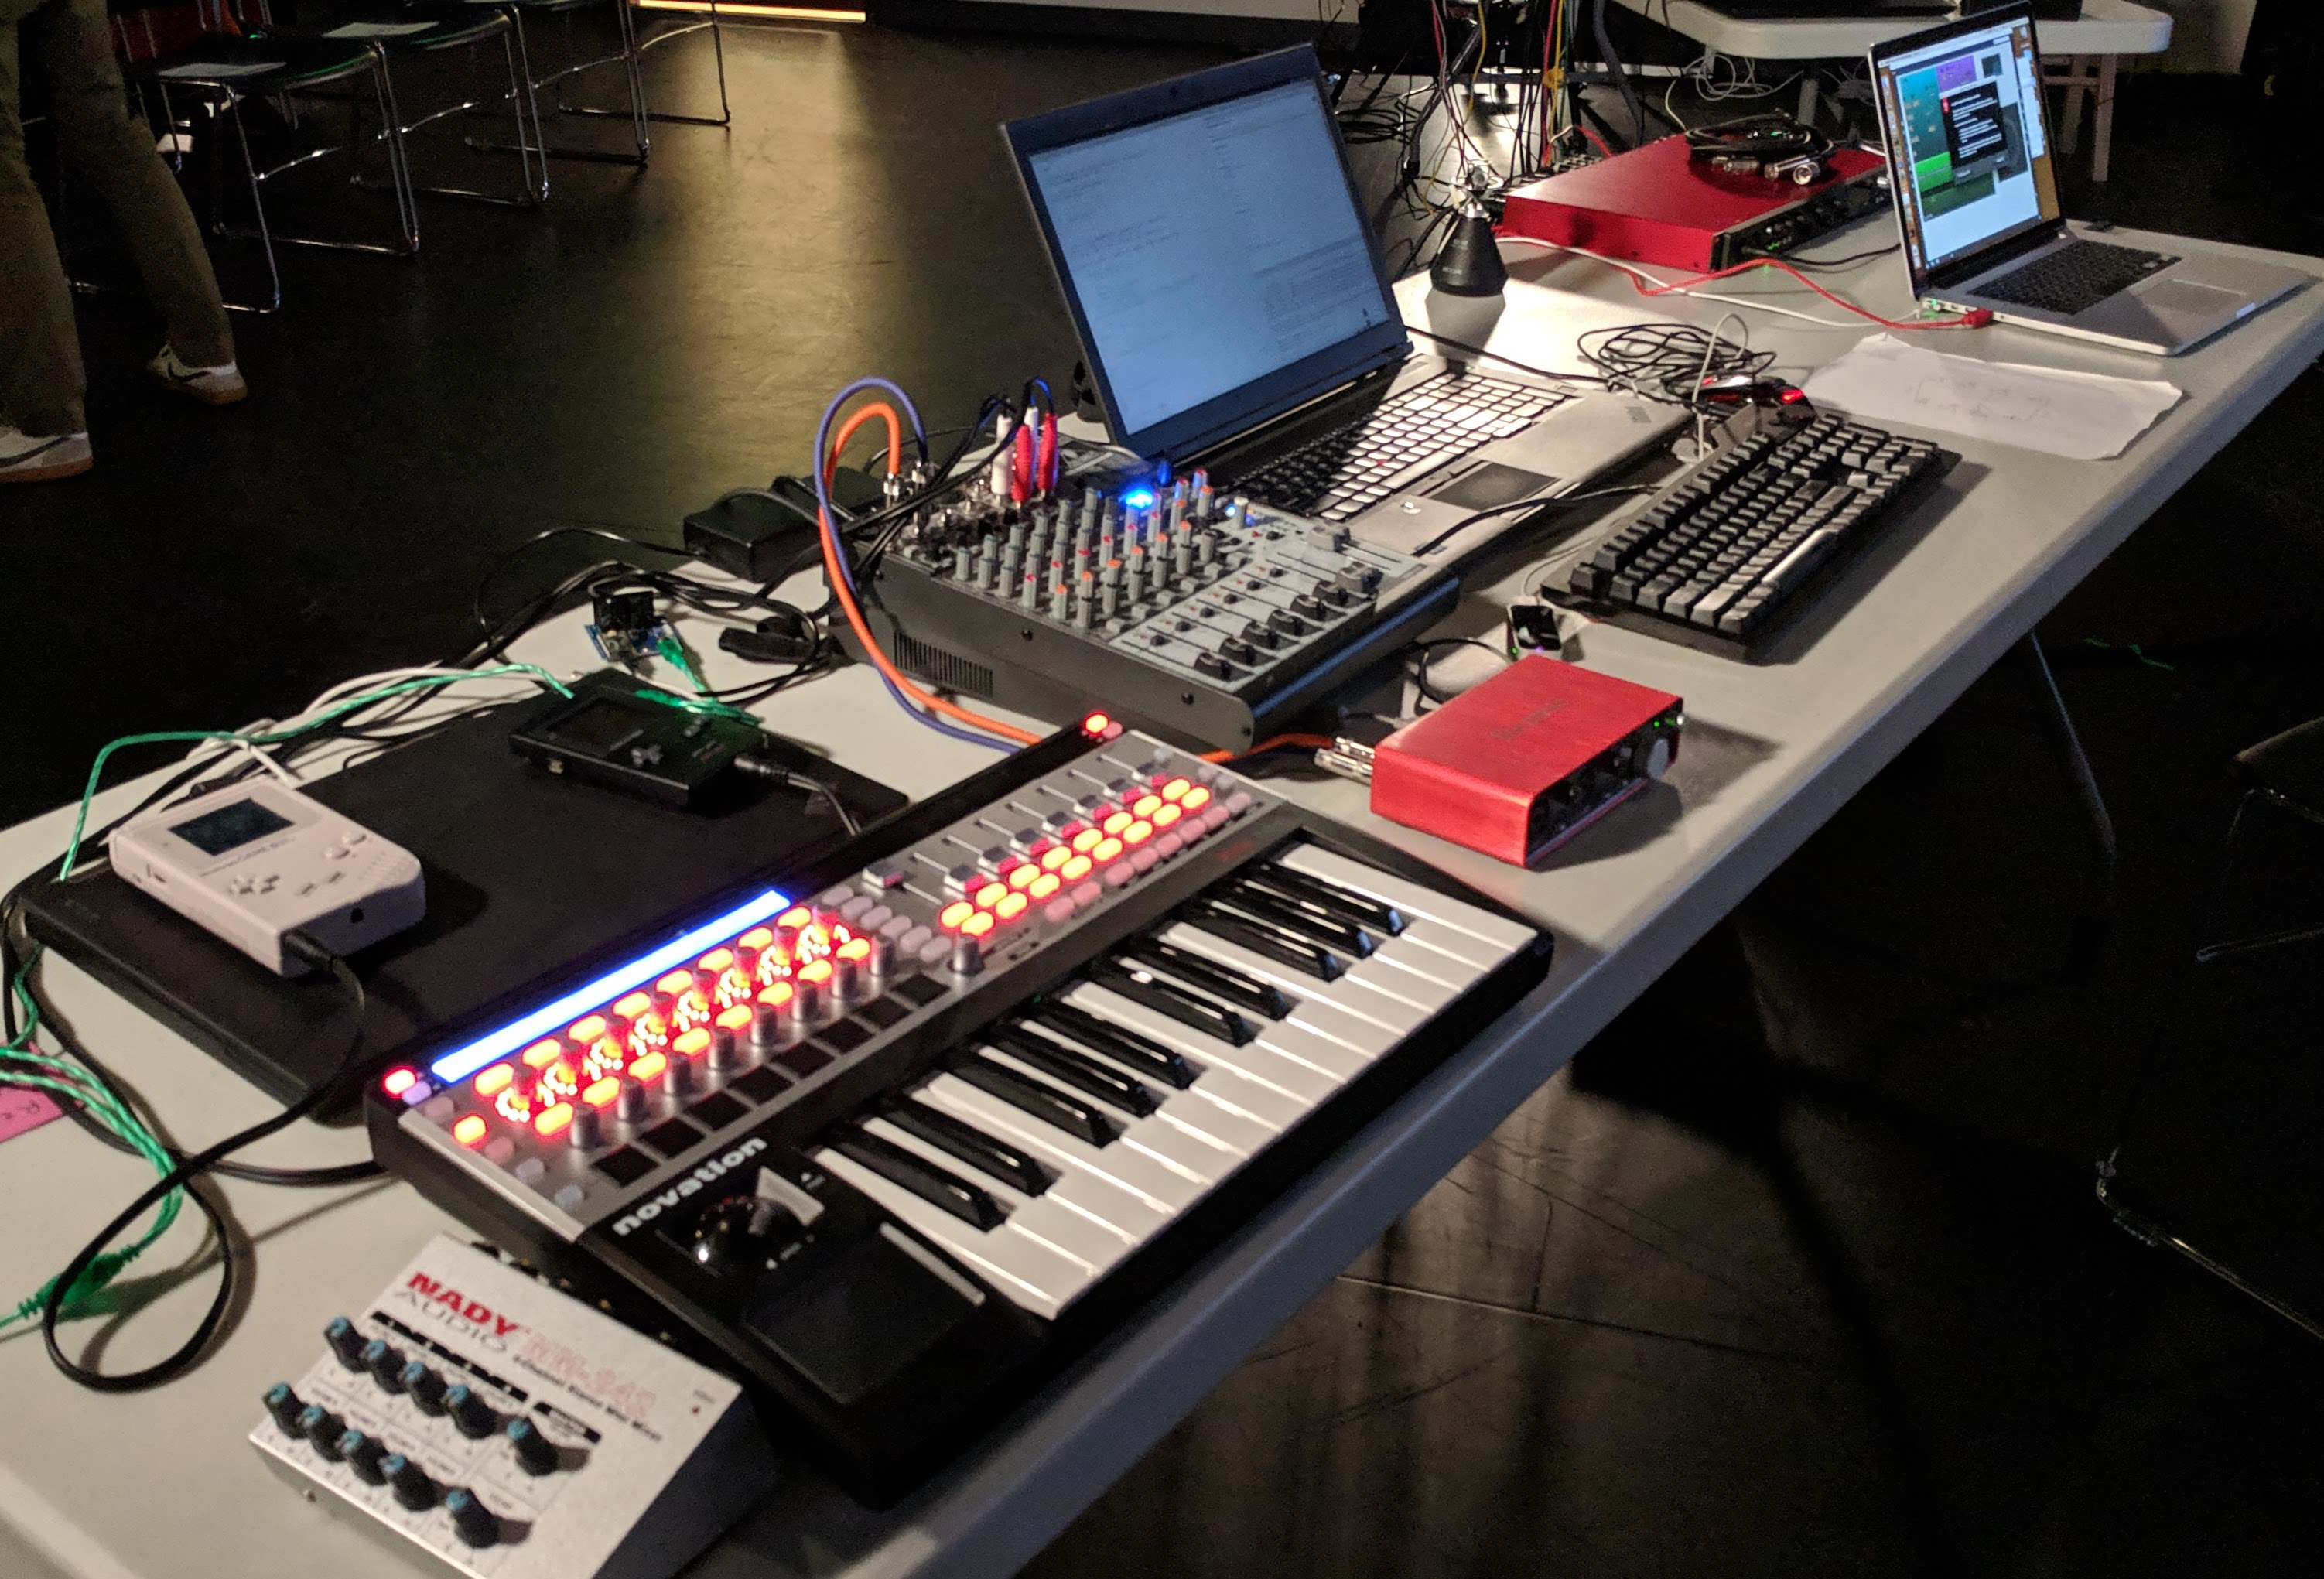
\includegraphics[width=0.85\columnwidth]{figs/concert.jpg}
    \caption{OMI using the CCAM space for a concert}
    \label{fig:concert}
\end{figure}

The OMI membership designs and coordinates a series of workshops that are offered over the course of the academic year at both the introductory and advanced level. Attendees typically consist of students from across the schools at Yale, faculty, staff, and local artists. In the workshops, OMI members introduce relevant concepts and technologies in topics. In the fall of 2018, topics included: building an LM386 amplifier circuit, basic theory of DSP and DSP programming in JUCE~\cite{juce}, hacking ``found'' hardware, and an introduction to Arduino and sensor networks.


 
\begin{figure}
    \centering
    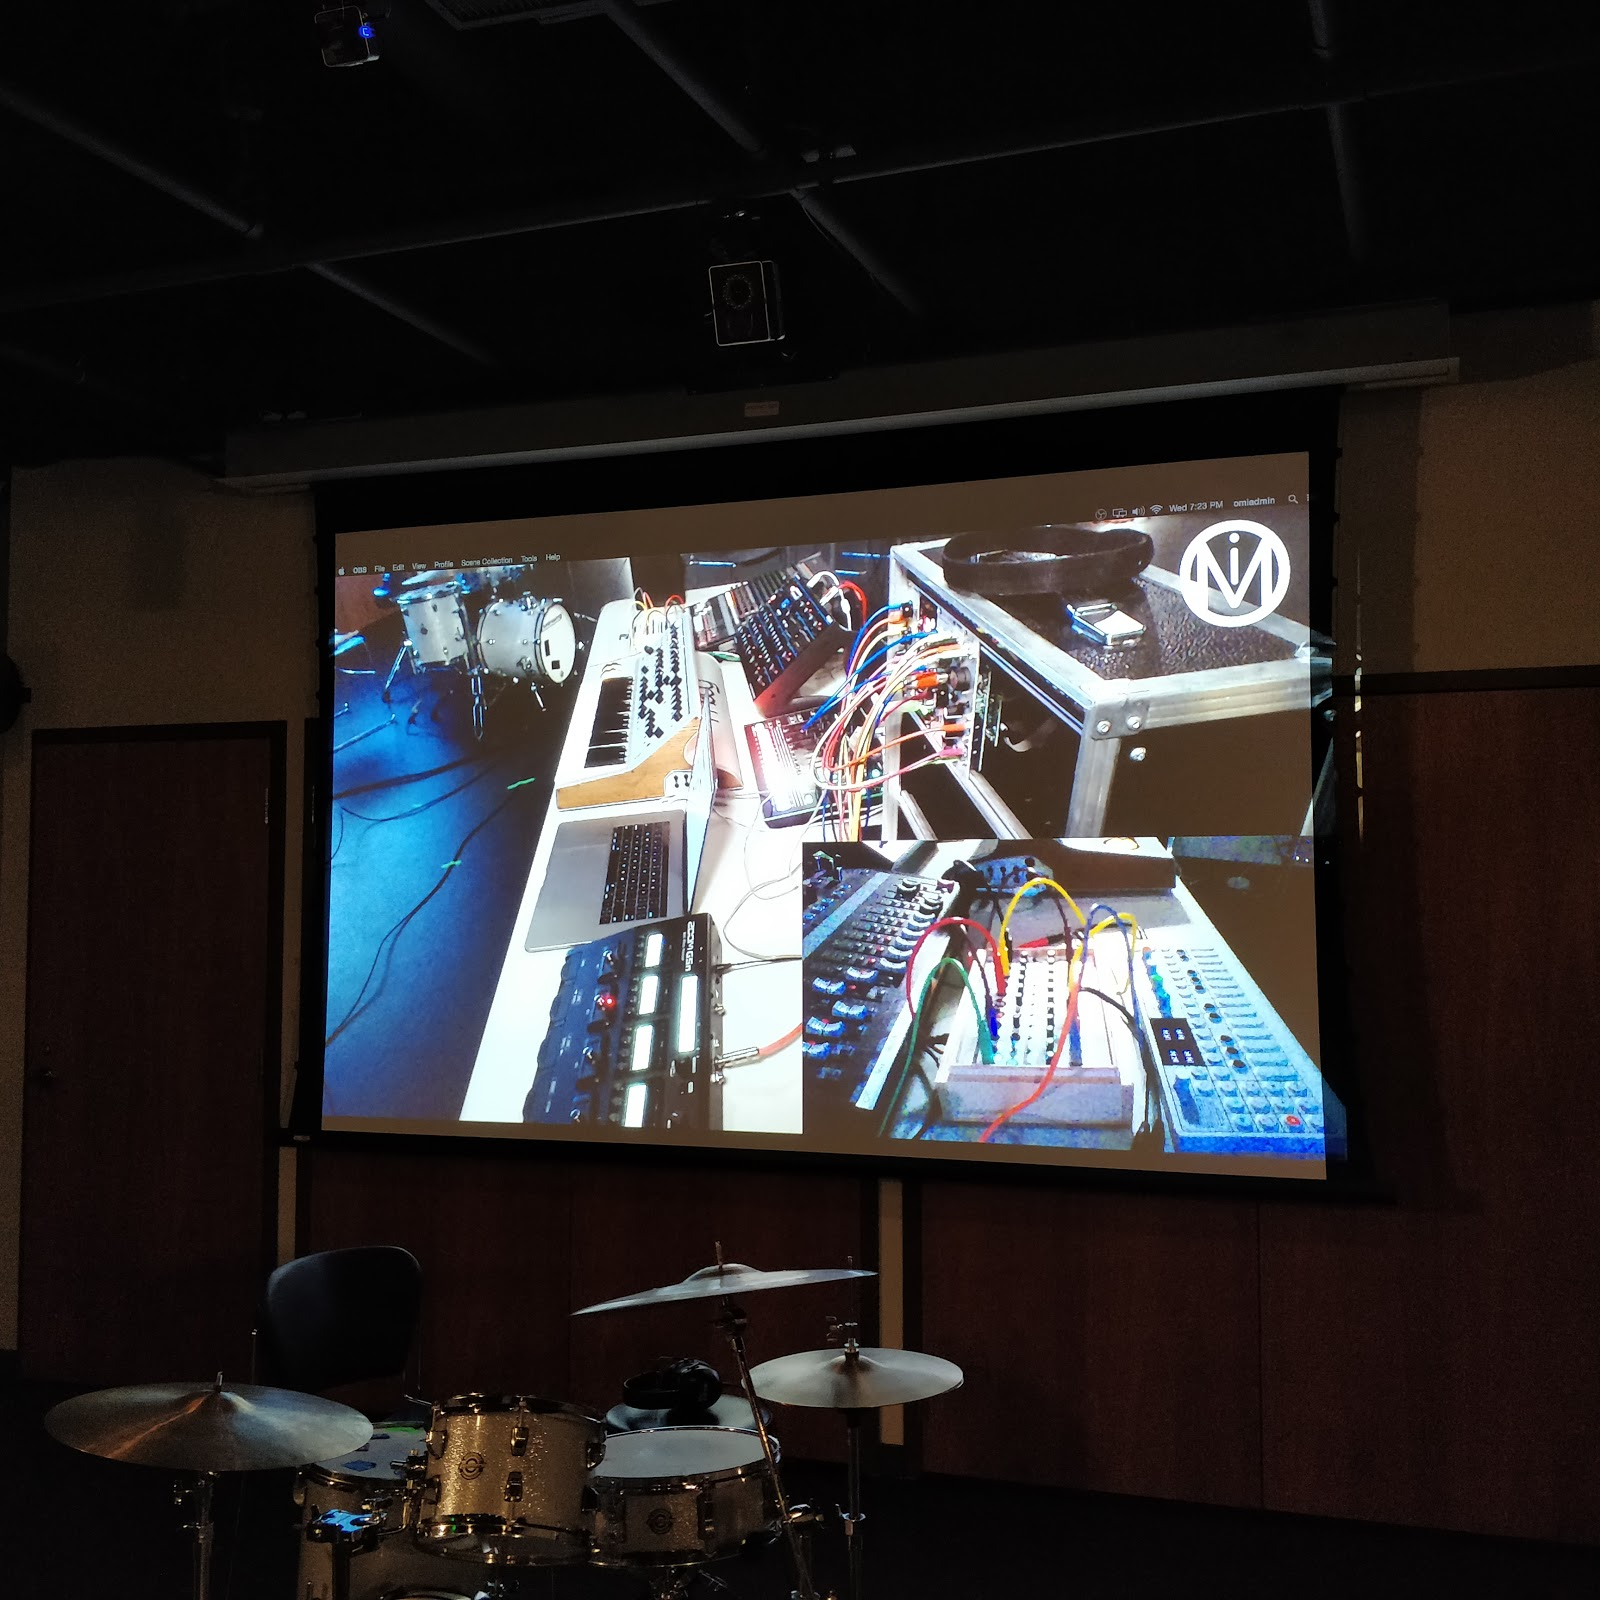
\includegraphics[width=0.85\columnwidth]{figs/concert2.jpg}
    \caption{OMI's end of semester concert}
    \label{fig:concert}
\end{figure}
 
In December 2018, OMI hosted a computer music concert showcasing work from students and faculty in the CCAM. The concert featured live electronics improvisation using analog and digital synthesizers, live coding, performances with interactive processing, and pieces utilizing eight-channel sound spatialization. A selection of the hardware used for this concert is shown in Fig.~\ref{fig:concert}.

